\clearpage
\section{Material e Métodos}\label{sec:methods}

Este capítulo aborda o protocolo de aquisição das imagens utilizadas para a análise e validação da proposta desse trabalho.
O conjunto de dados é o mesmo empregado em trabalhos relacionados, o que facilita a comparação da técnica desenvolvida com outros resultados encontrados na literatura.
Os recursos computacionais necessários para a implementação também são discutidos, com a finalidade de contribuir de forma transparente com a comunidade científica e facilitar a replicabilidade desse trabalho por interessados.
Nesse sentido, toda a implementação e dados usados nos experimentos foram disponibilizados em um repositório público\footnote{\url{github.com/sswellington/2PLA}} e podem ser obtidos por quaisquer usuários cadastrados no repositório.

O capítulo se foca nos métodos desenvolvidos para a segmentação das úlceras em membros inferiores que foram construídos e testados de forma próxima a incremental.
Em um primeiro momento, foi desenvolvida uma solução \textit{ad-hoc}, baseada exclusivamente em técnicas de processamento de baixo nível que se mostraram capazes de alcançar resultados interessantes para a separação entre fundo e pele.
A abordagem \textit{ad-hoc} foi avaliada em um pequeno conjunto de três imagens ulceradas e os resultados indicaram que uma solução estruturada, orientada a aprendizado de máquina, teria uma possibilidade de melhorar ainda mais o sucesso obtido.

Nesse sentido, em um segundo momento, foi proposta uma solução para segmentação de úlceras como uma abordagem em duas fases.
A primeira delas é baseada em classificação e permite separar fundo e pele, lesionada ou não.
Já a segunda parte possibilita aglutinar pedaços de tecidos similares que podem ser divididos entre lesão, cicatrização, pele saudável e outros.
As próximas seções apresentam a abordagem \textit{ad-hoc}, os resultados obtidos para segmentação e indícios de adequabilidade para o uso de técnicas de aprendizado de máquina e, finalmente, o método em duas fases proposto para a segmentação completa de úlceras.


\subsection{Material: Conjunto de Dados e Ferramentas}

Nesse trabalho foi usado o conjunto \dataset, gerado por \citeonline{Dorileo2008} e \citeonline{Pereira2011}.
Esse conjunto de imagens foi coletado de pacientes não-parentes por dermatologistas do Hospital das Clínicas da Universidade de São Paulo em Ribeirão Preto/SP (HC-FMRP-USP).
As fotografias coloridas de úlceras foram padronizadas de acordo com duas características: 
\textit{(i)}~plano de fundo -- foi usado um pano ou azul ou branco, e 
\textit{(ii)}~uma régua de cores.
A cor escolhida para o plano de fundo tem a finalidade de proporcionar contraste entre a pele do paciente e o fundo da imagem, de maneira a simplificar a tarefa de segmentação em uma técnica parecida com a \textit{croma key}.
Já a régua de cor foi usada com a finalidade de permitir a calibragem das cores em diferentes equipamento de projeções~\cite{Pereira2011}.

As imagem resultantes, no entanto, apresentam diversas dificuldades para o processamento.
Por exemplo, o fundo da imagem, ainda que azul ou branco, apresenta oscilação nas tonalidades de ``azul'' e ``branco'' e há uma irregularidade relacionada a distância da câmera ao membro inferior e o foco em torno das fotografias.
A câmera digital utilizada para obtenção das imagens foi a da fabricante Canon Inc, modelo  EOS 5D0, com a seguinte caracterização: Dois megapixels, lente macro de 50 mm e um filtro de polarização. 
A imagem resultante desta câmera possui tamanho de $1747\times1165$ \textit{pixels} com 24-bits de profundidade~\cite{Dorileo2008}.\\

\noindent
\textbf{Características do conjunto de dados.}
O conjunto de imagens, \dataset, utilizado contém $217$ fotografias de úlceras em membros inferiores com tamanhos variados e em estágios distintos de tratamento tiradas de pacientes anônimos com diferentes cores de pele, idade e sem parentescos entre si. 
Essa base imagens também foi construída e analisada em outros trabalhos~\cite{Dorileo2010,Pereira2011} com o objetivo de se identificar propriedades das lesões.
Para se comparar a qualidade das técnicas de análise, dermatologistas do HC-FMRP-USP segmentaram manualmente todas as $217$ imagens, gerando um conjunto de validação rotulado real -- um \textit{ground-truth} de validação.
Como resultado, milhões de \textit{pixels} estão rotulados em classes como, por exemplo, ``Fundo'' e ``Pele''.
Além disso, regiões de interesse foram divididas em tecidos lesionados e ao redor da úlcera que incluem partes de pele saudável, granulação, fibrina, necrose e mistura dos tecidos anteriores.
Todos os experimentos desse trabalho serão realizados em cima do \dataset e sua contraparte manualmente segmentada.
A Figura~\ref{fig:dataset_esp} apresenta um exemplo de uma imagem do conjunto \dataset e sua segmentação.\\

\begin{figure}[!htb]
\centering
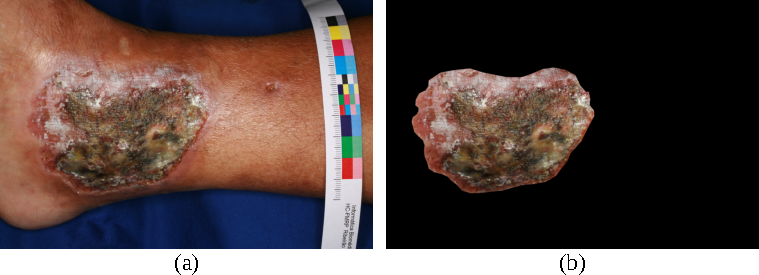
\includegraphics[scale=1]{_fig/im_sampling_vs_im_label.pdf}
\caption[Exemplo do conjunto de dados \dataset.]{Exemplo do conjunto de dados \dataset.
(a)~Imagem original.
(b)~Imagem segmentada pelo especialista.}
\label{fig:dataset_esp}
\end{figure}

\noindent
\textbf{Ferramentas.}
A análise do conjunto de dados depende do uso de ferramentas computacionais para a implementação dos métodos propostos.
Em particular, nesse trabalho, foram adotados os seguintes ambientes de desenvolvimento para implementação das abordagens discutidas:

\begin{itemize}
    \item \underline{Linguagem de desenvolvimento e IDE:} Weka\footnote{\url{cs.waikato.ac.nz/ml/weka/}} e Matlab R2018a Student\footnote{\url{mathworks.com/academia/students.html}}.
    \item \underline{Sistema de versionamento de código:} Git\footnote{\url{git-scm.com}}.
    \item \underline{Edição de imagens:} Gimp\footnote{\url{www.gimp.org/}} e Inkscape\footnote{\url{inkscape.org/}}.
    \item \underline{Geração de gráficos:} Gnuplot\footnote{\url{gnuplot.info/}}.
\end{itemize}

\subsection{Uma solução \textit{ad-hoc} para segmentação de pele e fundo}

Uma abordagem direta para segmentar as úlceras em membros inferiores é aplicar a técnica de limiarização de Otsu, seguida por técnicas de morfologia para suavização das bordas e eventual remoção de pixels ruidosos.
Não obstante, o primeiro desafio que surge \textit{antes} da aplicação do método de limiarização é a transformação da imagem em uma representação monocromática.
Uma solução direta é a conversão da imagem de 24-bits em uma imagens em tons de cinza de 8-bits.
Essa abordagem direta se mostrou inadequada na prática, por duas razões:
\textit{(i)}~a quantidade de pixels de fundo é muito maior que a quantidade de pixels de pele e influencia a média e variância do método de limiarização e
\textit{(ii)}~a tonalidade de fundo, quando convertida para escala de cinza, perde parte da sua capacidade discriminativa.
A Figura~\ref{fig:conv_falha} apresenta um contra exemplo para essa abordagem.

\begin{figure}[!htb]
\centering
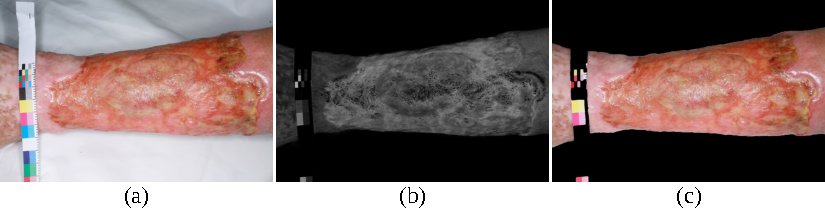
\includegraphics[scale=1.15]{_fig/otsu_phase.pdf}
\caption[Limiarização direta de conversão de imagem monocromática]{Limiarização direta de conversão de imagem monocromática.
(a)~Imagem original.
(b)~Imagem monocromática.
(c)~Limiarização de Otsu.}
\label{fig:conv_falha}
\end{figure}

De acordo com esse resultado, para se obter a transformação da imagem original em monocromática, foram testados diversos pesos, escolhidos de maneira \textit{ad-hoc}, para ponderar e converter as componentes RGB em escala de cinza.
Após testes com esse conjunto de pesos candidatos, o resultado que apresentou o melhor resultado para converter um pixel $P_i$ de 24-bits em um pixel $P_i'$ unidimensional foi o da fórmula da Equação~\ref{eq:pesos}.
Um exemplo passo-a-passo dessa conversão é ilustrado na Figura~\ref{fig:monocromatica}.

\begin{equation}\label{eq:pesos}
    P_i' = (r_i', g_i', b_i');~r_i' = g_i' = b_i' = r_i - \frac{g_i + b_i}{2}
\end{equation}

\begin{figure}[!htb]
\centering
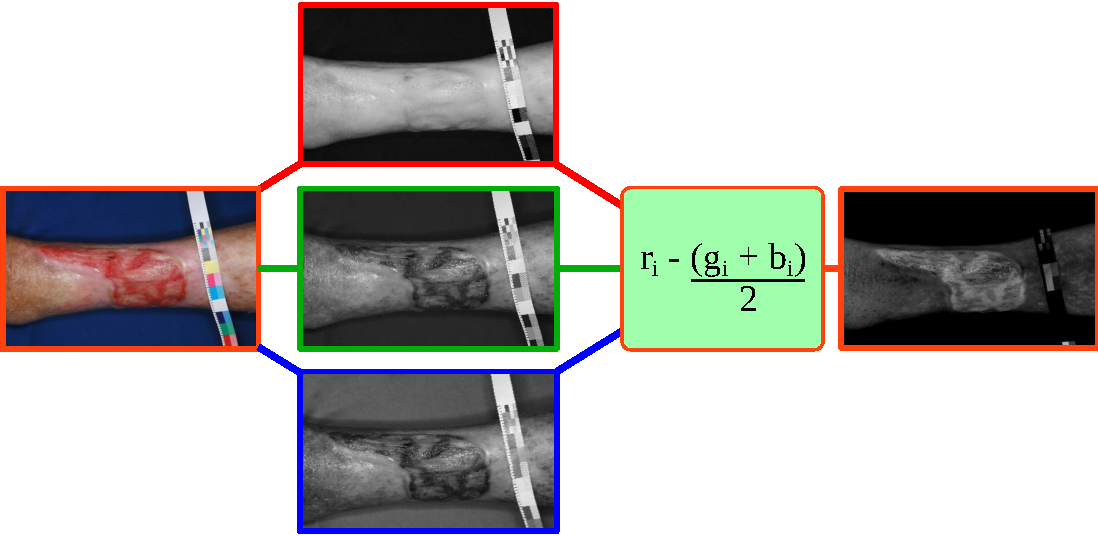
\includegraphics[scale=.75]{_fig/mono.pdf}
\caption[Pesos \textit{ad-hoc} de conversão 24-bits para monocromática]{Pesos \textit{ad-hoc} de conversão 24-bits para monocromática.}
\label{fig:monocromatica}
\end{figure}

\begin{figure}[b]
\centering
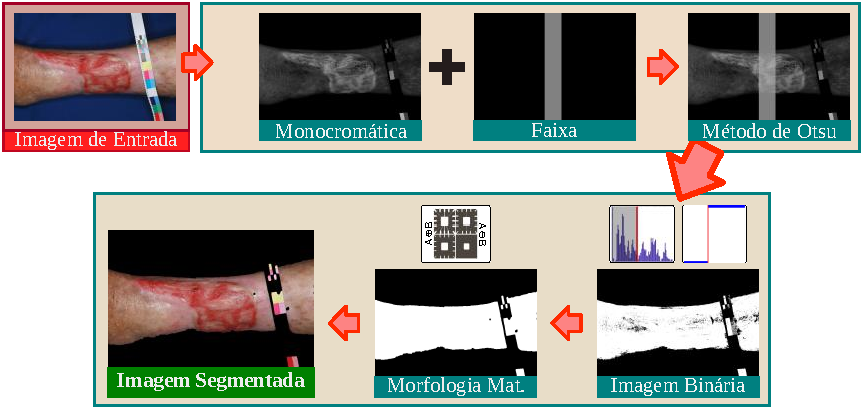
\includegraphics[scale=1.05]{_fig/pipelineAdhoc.pdf}
\caption[Solução de segmentação \textit{ad-hoc}]{Solução de segmentação \textit{ad-hoc}.}
\label{fig:systemAdhoc}
\end{figure}

A partir da conversão sugerida da imagem 24-bits para a imagem monocromática, o desafio torna-se reduzir a influência dos pixels de fundo no método de limiarização.
Nesse sentido, optou-se por usar uma faixa vertical centralizada de $10\%$ da largura da imagem original como uma janela fixa para a construção do histograma do método de Otsu.
O ponto de corte, então, passa a ser delimitado pelos pixels dentro dessa janela.
Ao final da limiarização é possível que a imagem binária apresente pixels incorretamente mantidos e que podem ser removidos por intermédio da morfologia matemática.
Ao se comparar as operações morfológicas revisadas, o operador da abertura foi o que conseguiu remover mais pixels ruidosos.

\begin{algorithm}[!b]
\nonl \rule[0.5ex]{410px}{0.5pt}\\
\SetKwFunction{mono}{MONOCROMATICA}
\SetKwFunction{faixa}{FAIXA}
\SetKwFunction{otsu}{OTSU}
\SetKwFunction{bin}{binaria}
\SetKwFunction{morph}{MORFOLOGIA\_MATEMATICA}
\SetKwInOut{Input}{Entrada}
\SetKwInOut{Output}{Saída}
 \Input{Imagem $I$.}
 \Output{Tecidos segmentados de pele (lesionados ou não).}
\nonl \rule[0.5ex]{410px}{0.5pt}\\

$I' \leftarrow$ \mono{$I$};\tcc{Tons de cinza}
$histograma \leftarrow$ \faixa{$I'$};\tcc{Amostragem de pixels}
$mascara \leftarrow$ \otsu{$I', histograma$};\tcc{Limiarização}
$I' \leftarrow I' - mascara$\;
$I' \leftarrow$ \morph{$I'$};\tcc{Fechamento e abertura}
$I' \leftarrow I - I'$\;
\Return $I'$\;
\nonl \rule[0.5ex]{410px}{0.5pt}\\
\caption{Algoritmo para implementação da solução \textit{ad-hoc}.}
\label{alg:ad-hoc}
\end{algorithm}

A concatenação das operações de 
\textit{(i)}~transformação monocromática,
\textit{(ii)}~amostragem por janela vertical fixa,
\textit{(iii)}~método de Otsu e 
\textit{(iv)}~morfologia matemática de abertura permite obter uma máscara para a imagem original que descarta o plano de fundo da imagem, restando apenas a pele do paciente.
O passo-a-passo dessa solução em sequência \textit{ad-hoc} é descrita pelo Algoritmo~\ref{alg:ad-hoc} e, visualmente, pela Figura~\ref{fig:systemAdhoc}.



\begin{figure}[!htb]
\centering
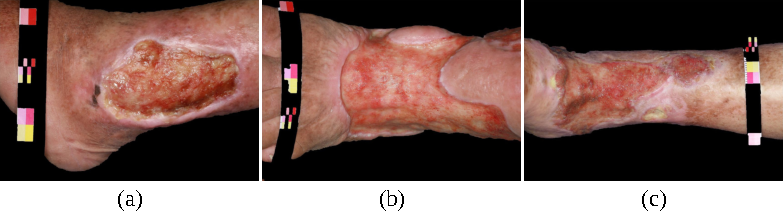
\includegraphics[scale=1.2]{_fig/otsu_result.pdf}
\caption[Três exemplos de imagens segmentadas de acordo com a solução \textit{ad-hoc}]{Três exemplos de imagens segmentadas entre fundo e pele, de acordo com a solução \textit{ad-hoc} de processamento de baixo nível.}
\label{fig:res_adhoc}
\end{figure}

Foram realizados experimentos com três imagens do conjunto \dataset que foram segmentadas pela solução \textit{ad-hoc} e comparadas com a segmentação gerada manualmente pelos especialistas.
A Figura~\ref{fig:res_adhoc} apresenta os resultados para três imagens geradas pelo Algoritmo~\ref{alg:ad-hoc}.
O resultado indica que alguns pixels foram perdidos pela solução \textit{ad-hoc}.
Ainda que o processo de limiarização tenha sido bastante refinado, ele ainda é responśavel por definir apenas um \textit{único} ponto de corte.
Tonalidades de cores que estejam agrupadas por intervalos, portanto, não são diferenciadas pela estratégia da limiarização, pois o valor de corte é incapaz de dividir as tonalidades em mais de um conjunto usando diversos limitantes de menor e maior valor.

Essa limitação do procedimento baseado na limiarização por Otsu é facilmente contornada pelo uso de um algoritmo classificador.
Em especial, algoritmos de classificação que operem com um viés de aprendizado capaz de definir múltiplos pontos de corte na reta de tonalidades de 8-bits (ou ainda \textit{planos} de corte para tonalidades de 24-bits) são particularmente adequados para tratar essa característica do problema de separação de pele e fundo.
Nesse sentido, redes neurais artificiais (que geram planos de corte) ou árvores de decisão (que geram hiper-retângulos de corte) são métodos com possibilidade de apresentar boa aderência ao problema.


\subsection{Abordagem de Aprendizado em Duas Fases}

Baseado nos resultados observados da aplicação da solução \textit{ad-hoc} de baixo nível, foi proposta uma segunda solução totalmente orientada ao aprendizado de máquina, que realiza processamento de médio e alto nível, para a segmentação de úlceras em membros inferiores.
A separação entre pele e fundo foi tratada com um problema de \textit{classificação} e, devido aos bons resultados, foi projetada também uma segunda fase, que consiste em \textit{agrupar} superpixels somente de pele em regiões similares.

Em particular, para o projeto da segunda fase, foram seguidas indicações encontradas em trabalhos relacionados.
Primeiro, o uso de superpixels como abordagens de divisão-e-conquista são relatados como abordagens eficientes para separar tecidos saudáveis de lesionados.
Ainda nesse sentido, o uso de técnicas de agrupamento e não as de classificação de superpixels parecem as mais indicadas para lidar com o problema de diferentes tipos de tecidos encontrados em regiões lesionadas.
O uso de técnicas de agrupamento permite manter informações, ao invés de descartá-las como não relevantes.
Por exemplo, agrupar o tecido saudável ao redor da úlcera pode ser útil para indicar se o procedimento de cicatrização está sendo acelerado ou devagar demais no contexto de um determinado tratamento indicado pelo dermatologista -- uma informação que seria descartada caso um classificador fosse empregado para rotular o tecido como simplesmente lesionado ou não-lesionado.

Portanto, o projeto da solução combina as duas fases de aprendizado supervisionado e não-supervisionado para alcançar uma segmentação de úlceras que seja capaz de descartar apenas informações irrelevantes para o problema, \textit{i.e.}, pano de fundo usado na fotografia, e manter as informações úteis no contexto da lesão, organizadas de acordo com um critério de similaridade.
Uma vez que a solução é dividida nessas duas partes, foi dada a ela o nome de \system (\textit{Two-Phase Learning Approach}), ou Abordagem de Aprendizado em Duas Fases.

\begin{figure}[!htb]
\centering
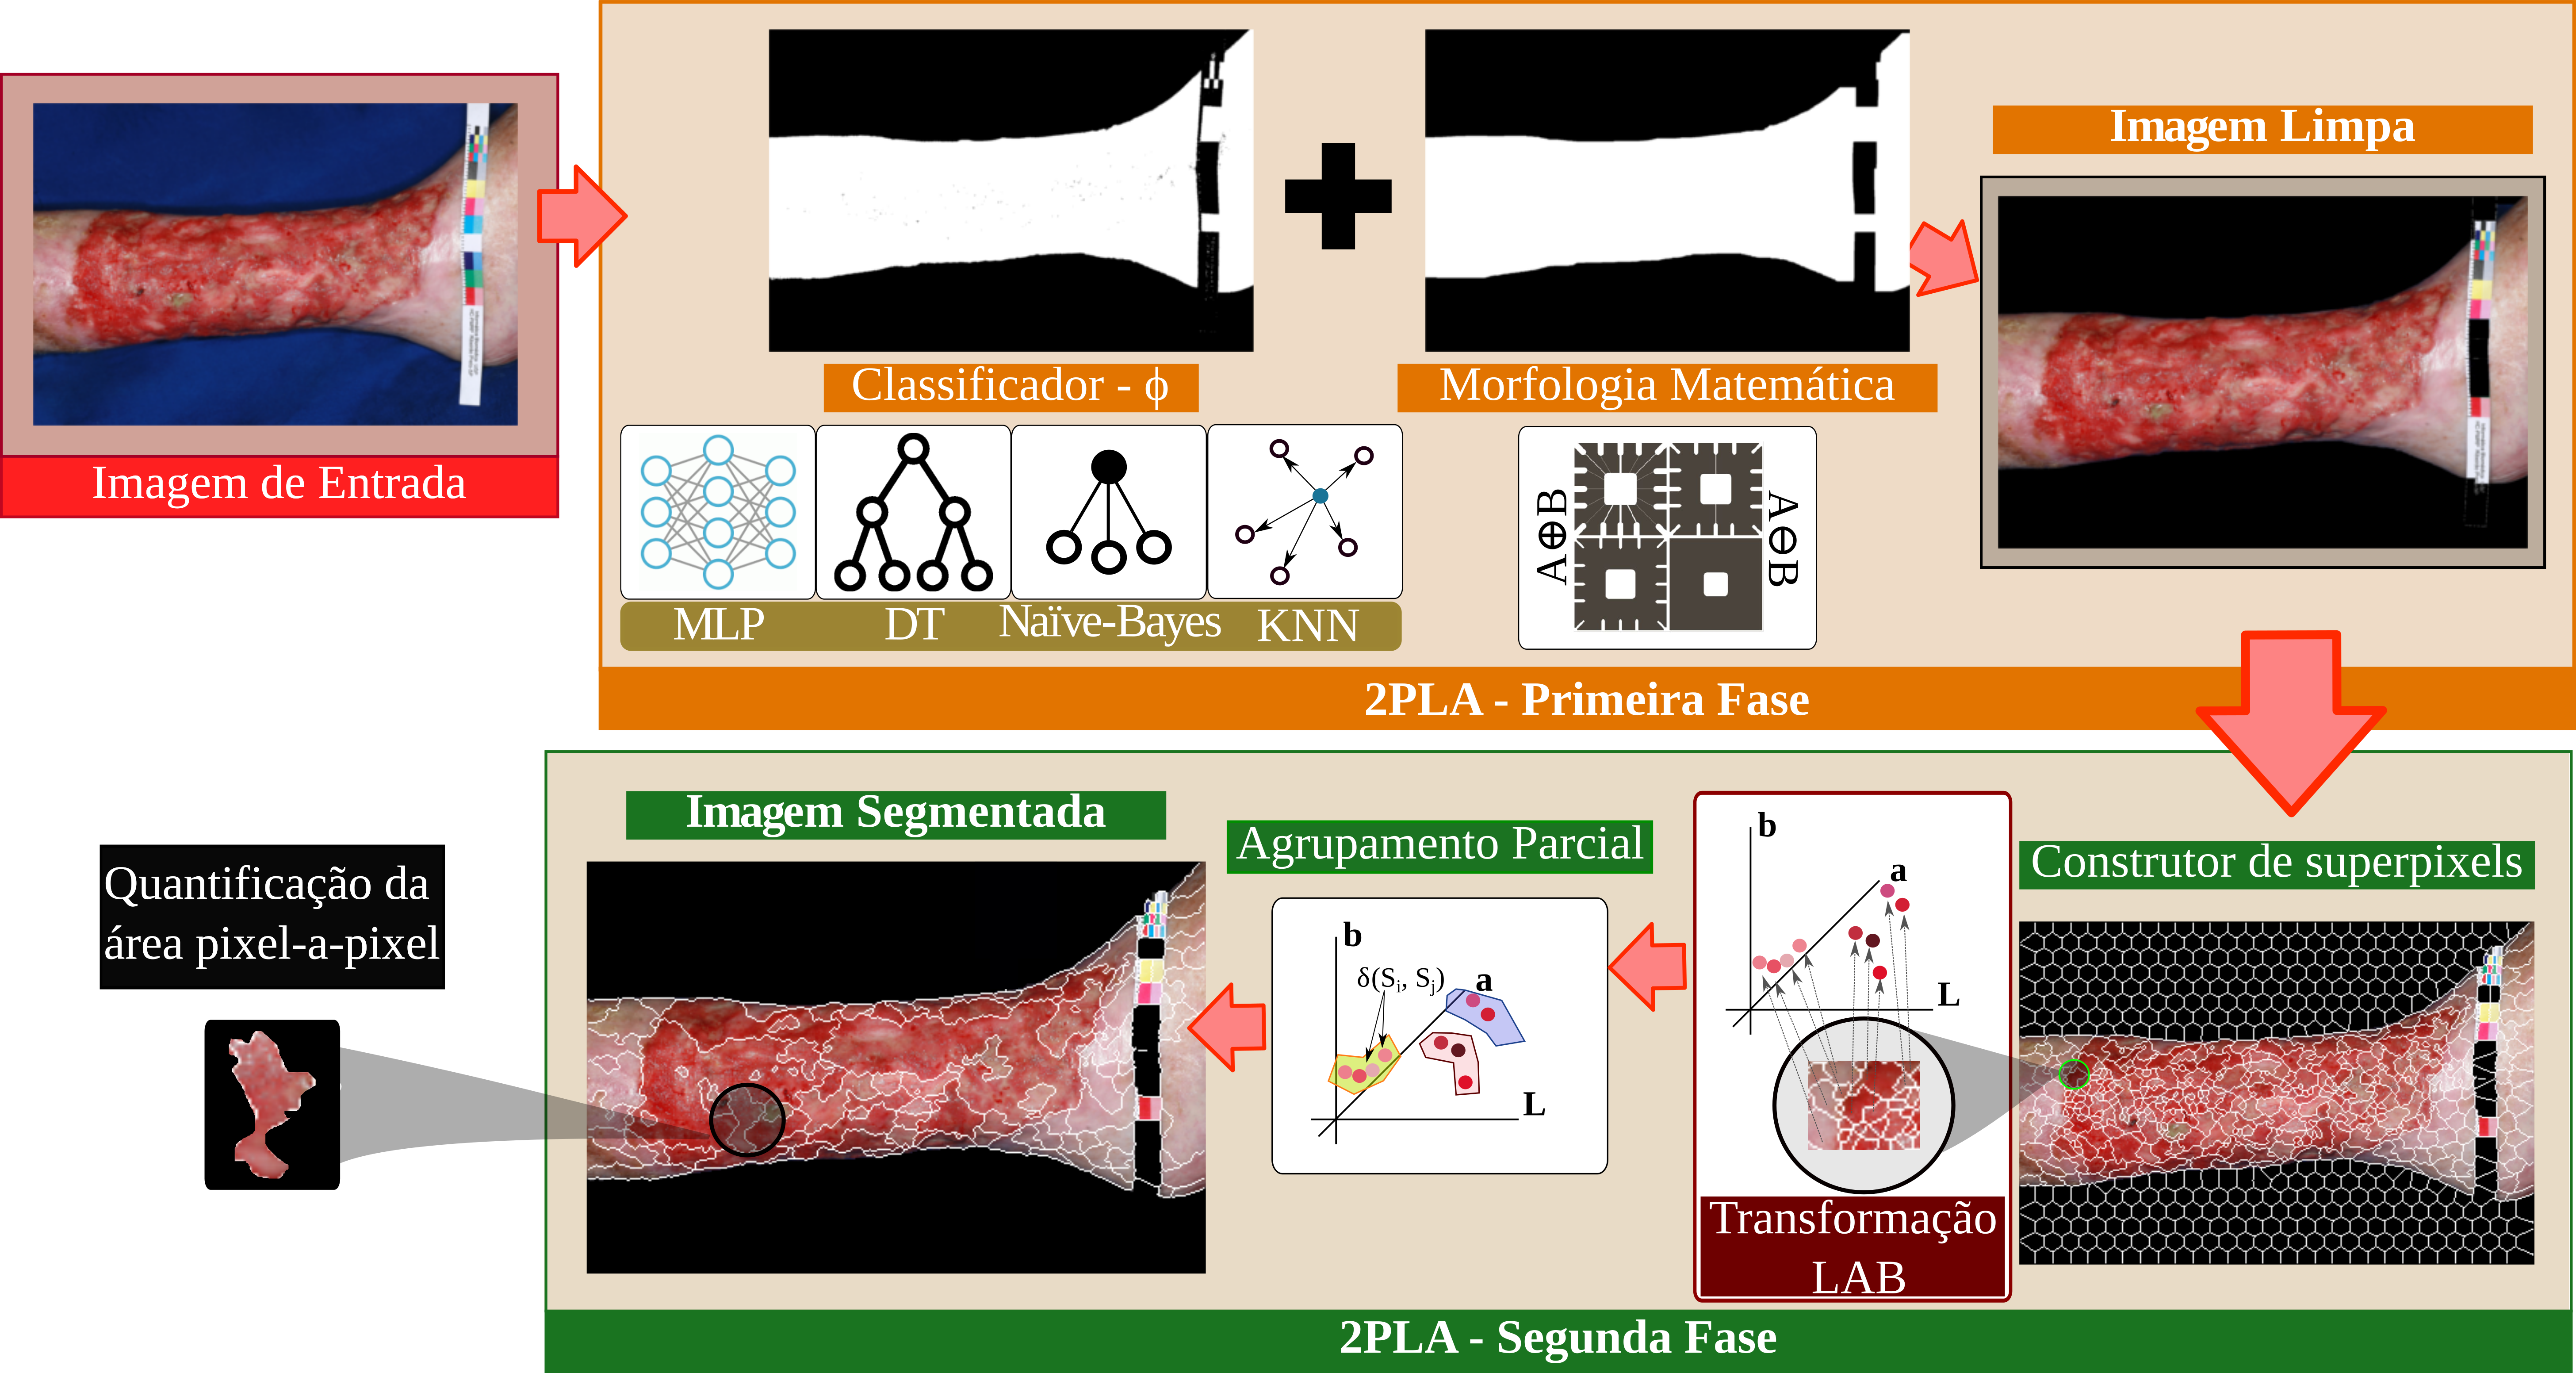
\includegraphics[scale=.63]{_fig/pipeline.png}
\caption[Sequência de processamento da solução \system]{Sequência de processamento da solução \system.
A primeira fase remove os pixels de fundo, por meio de ma classificação pixel-a-pixel diretamente no espaço de cores RGB.
Eventuais remoções indevidas e pixels ruidosos são restaurados com o apoio da morfologia matemática.
As imagens ``limpas'' são divididas em superpixels e representadas no espaço de cores LAB, que é mais adequado para representar a noção de distância entre as cores.
Na sequência, a segunda fase aplica um algoritmo de agrupamento particional para nos os superpixels semelhantes em regiões únicas.
As fronteiras dessas regiões são colocadas sobre a imagem original para gerar uma máscara de segmentação para cada pixel. 
Assim, a área dos tecidos segmentados pode ser quantificada com relação ao número de seus \textit{pixels}.}
\label{fig:system}
\end{figure}

A Figura~\ref{fig:system} apresenta todos os estágios e subdivisões da solução \system.
A primeira fase, de classificação, possui o objetivo de descartar o fundo da imagem de modo que permaneça apenas a pele do paciente.
Para isso, remove-se os pixels de fundo através de sua classificação como relevante ou não, o que requer um conjunto rotulado de pixels para treinamento prévio do classificador.
Para gerar esse conjunto foram usadas as segmentações \textit{ground-truth} do \dataset considerando cinco imagens diversificadas entre si, \textit{i.e.}, fundo azul e branco, diferentes tons de pele e membros ulcerados, e dois possíveis rótulos $L = \{$Pele, Fundo$\}$.
Após a classificação pixel-a-pixel, o método \system aplica a morfologia matemática e também o filtro de mediana para correção de pixels ruidosos e geração da máscara de remoção de fundo.
O elemento estruturante, usado na operação morfológica é um retângulo proporcional à imagem de entrada, cujo perímetro equivale à $1\%$ da imagem original.
O resultado desse processo, resulta em imagens ``limpas'' (sem fundo), que servem para alimentar a segunda fase.


Nesse ponto, a imagem é dividida em superpixels para criar uma ``malha'', sendo empregado para essa tarefa o método SLIC.
Acompanhando os resultados da literatura que indicam 550 como um bom número de superpixels para o conjunto de dados \dataset, definiu-se uma função para variar a quantidade de superpixels fornecida ao SLIC em razão do perímetro das imagem e o valor $550$.
Nesse sentido, se as imagens fornecidas para processamento forem de tamanho diferente das imagens do conjunto \dataset, a quantidade de superpixels gerada pelo \system pode ser maior ou menor que $550$ para melhor se ajustar à imagem de entrada.
Os superpixels gerados são representados em três dimensões RGB de acordo com a Definição~\ref{def:superpixel} e, então, convertidos às coordenadas LAB.
Essa conversão é importante, pois o algoritmo de agrupamento usa uma função de distância para medir a similaridade entre os superpixels, sendo que o espaço LAB é mais indicado para representar as distâncias entre as cores, do ponto de vista da intuição geométrica de distância, do que o espaço RGB.

Na sequência, a segunda fase aplica um método para agrupar os \textit{superpixels} e as regiões unidas geram uma máscara, agora capaz de identificar tecidos com características distintas.
O método \system usa o algoritmo DBSCAN para criar os grupos, pois esse algoritmo não requer especificar a quantidade de \textit{clusters} esperada ao final do agrupamento.
Ao invés disso, apenas a distância e a densidade de elementos são levadas em consideração para unir os superpixels similares.
No final do processo de agrupamento, os superpixels são unidos em uma única porção de tecido, que pode ter a sua área quantificada com relação ao número de pixels internos e a totalidade de pixels da imagem original.
Por exemplo, se uma região de uma imagem do conjunto \dataset apresenta $5 \cdot 10^3$ pixels, então a área da região é dita $5 \cdot 10^3/ (1747 \times 1165) \approx 0,002$, ou ainda $0,2\%$ da imagem original.
Caso exista a equivalência do plano da fundo em $c_q$ centímetros quadrados, então a área da lesão pode ser imediatamente estimada como $0,002 \cdot c_q$ cm$^2$, o que permite ao especialista acompanhar se o tecido lesionado está aumentando ou diminuindo quando duas fotografias em momentos diferentes são comparadas.
Além disso, o especialista pode rapidamente rotular os conjuntos de tecidos similares agrupados entre saudável, fibrina, granulação, necrose ou ainda uma mistura dos tecidos.
Esse procedimento de rotulagem é facilitado pois, ao invés do especialista definir as regiões de fronteira e/ou classificar milhares de pixels, apenas alguns poucos superpixels serão retornados ao final do processo \system.
No caso das imagens do conjunto \dataset, por exemplo, certamente serão retornados menos do que $550$ regiões de interesse/superpixels agrupados.

O Algoritmo~\ref{alg:2pla} implementa a rotina principal do método \system e depende de um conjunto de parâmetros a serem fornecidos como entrada.
O parâmetro $k$ define o número de superpixels, e parâmetro $\phi$ é um classificador treinado para rotular pixels entre $L = \{$Pele, Fundo$\}$.
Os parâmetros $\delta$ e $\xi$ são configurações DBSCAN que definem como a similaridade entre dois superpixels é medida e o limite máximo de dissimilaridade, respectivamente.
É importante, portanto, destacar que o desempenho final da solução depende do ajuste da configuração de valores adequados para os parâmetros do Algoritmo~\ref{alg:2pla}.
Com relação a execução, a rotina se vale de marcar pontos de interesse de processamento através do pixel especial de descarte $P_a$ que tem valor RGB $(0, 0, 0)$.
O procedimento de classificação marca os pixels a serem descartadas como $P_a$ e os superpixels uniformes $S$ com valor $\bar{P}_S = P_a$ não são considerados pelo algoritmo de agrupamento.
A rotina de morfologia matemática faz o procedimento de fechamento e abertura, além da aplicação do filtro da mediana.
Finalmente, as fronteiras dos pixels agrupados são colocados sobre a imagem original.

\begin{algorithm}[!htb]
\nonl \rule[0.5ex]{410px}{0.5pt}\\
\SetKwFunction{slic}{SLIC}
\SetKwFunction{dbscan}{DBSCAN}
\SetKwFunction{morph}{MORFOLOGIA\_MATEMATICA}
\SetKwFunction{rgbTolab}{RGB\_TO\_LAB}
\SetKwInOut{Input}{Entrada}
\SetKwInOut{Output}{Saída}
\Input{Imagem $I$, função de distância métrica $\delta$, \textit{threshold} da similaridade $\xi$, número de superpixels $k$, e classificador treinado $\phi$.}
\Output{Tecidos segmentados dentro e ao redor da úlcera.}
\nonl \rule[0.5ex]{410px}{0.5pt}\\
$P_a \leftarrow \langle 0, 0, 0\rangle$\;
\tcc{Descarta pontos sem interesse}
\For{$P_i \in I$}{
    \If{$\phi(P_i) \neq$ ``Pele''}{
        $P_i \leftarrow P_a$\;
    }
} %For
$I \leftarrow$ \morph{$I$};\tcc{Fechamento e abertura}
$\mathcal{S} \leftarrow$ \slic{$I$, $k$}\;
\tcc{Descarta $S \in \mathcal{S}$ sempre que $\rgbTolab(\bar{P_S}) = \rgbTolab(P_a)$}
$\mathcal{S'} \leftarrow$ \dbscan{$\mathcal{S}, \delta, \xi$}\;
\Return $\mathcal{S'}$ sobre $I$\;
\nonl \rule[0.5ex]{410px}{0.5pt}\\
\caption{Implementação do método \system.}
\label{alg:2pla}
\end{algorithm}

\subsection{Conclusões Parciais}

Nessa seção foram apresentados os materiais, ferramentas e métodos usados para tratar o problema de segmentação de imagens de úlceras em membros inferiores.
Em particular, foi apresentado o conjunto de imagens de úlceras \dataset e as ferramentas empregadas para codificação da proposta desse trabalho final de curso.
Para além disso, de acordo com as indicações e conceitos revisados na Seção~\ref{sec:background}, duas alternativas de solução foram discutidas para o problema: uma primeira, baseada em processamento de imagens de baixo nível, e uma segunda, que é baseada no processamento de imagens de médio e alto nível.
No primeiro caso, projetou-se uma solução \textit{ad-hoc} que usa os conceitos de transformações de imagens \textit{full-color} para imagens monocromáticas, métodos de amostragem, limiarização pelo critério de Otsu e morfologia matemática.
Com a implementação da solução \textit{ad-hoc}, foram avaliados os resultados de três imagens do conjunto \dataset, que apresentaram boa separação entre fundo e pele, mas com perda de pixels em alguns trechos das imagens.

Após análise, verificou-se que o algoritmo de limiarização de Otsu gera apenas um único ponto de corte para separar pixels de pele e fundo e que alguns desses pixels não podem ser separados com apenas um valor limitante.
Nesse sentido, uma alternativa viável foi o desenvolvimento e proposta de uma solução orientada ao aprendizado de máquina, que foi denominada de \system.
Essa solução não apenas usa um classificador capaz de gerar múltiplos intervalos de corte e separa pixels de pele e fundo, mas também permite que a região classificada como pele seja subdividida em regiões de interesse.
Em particular, a imagem com fundo descartado é dividida em superpixels com bordas que aderem ao formato das regiões e que são unidos por meio de um algoritmo de agrupamento.
Assim, o especialista do domínio de úlceras pode analisar cada tecido em separado, bem como ter uma estimativa da área de cada uma das partes segmentadas da imagem.

No entanto, toda a solução \system depende de parâmetros de entrada que são fornecidos pelo usuário, tais como o método de classificação, um número inicial de superpixels, uma função de distância para medir a similaridade entre superpixels e um valor máximo de similaridade tolerado no agrupamento.
A escolha desses parâmetros é que, em última instância, determina a qualidade da solução \system.
Nesse sentido, uma série de avaliações experimentais foram realizadas para determinar qual a melhor configuração para a proposta orientada ao processamento de médio e alto nível.
A próxima seção detalha essas avaliações, bem como relata experimentos que visam medir a qualidade da segunda solução proposta nese capítulo.
\newpage
\thispagestyle{plain} % empty
\mbox{}


